% This file was created by matplotlib2tikz v0.6.15.
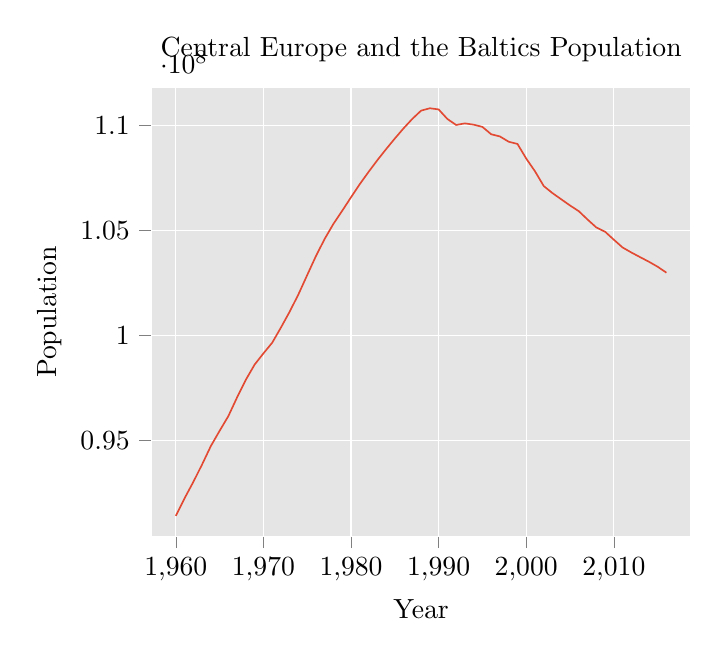
\begin{tikzpicture}

\definecolor{color0}{rgb}{0.886274509803922,0.290196078431373,0.2}

\begin{axis}[
title={Central Europe and the Baltics Population},
xlabel={Year},
ylabel={Population},
xmin=1957.2, xmax=2018.8,
ymin=90431593.15, ymax=111771369.85,
tick align=outside,
tick pos=left,
xmajorgrids,
x grid style={white},
ymajorgrids,
y grid style={white},
axis line style={white},
axis background/.style={fill=white!89.80392156862746!black}
]
\addplot [semithick, color0, forget plot]
table {%
1960 91401583
1961 92237118
1962 93014890
1963 93845749
1964 94722599
1965 95447065
1966 96148635
1967 97043587
1968 97882394
1969 98602140
1970 99133296
1971 99638983
1972 100363597
1973 101120519
1974 101946256
1975 102862489
1976 103770134
1977 104589313
1978 105304312
1979 105924838
1980 106564905
1981 107187982
1982 107770794
1983 108326895
1984 108853181
1985 109360296
1986 109847148
1987 110296680
1988 110688533
1989 110801380
1990 110745760
1991 110290445
1992 110005636
1993 110081461
1994 110019570
1995 109913216
1996 109563097
1997 109459093
1998 109207205
1999 109102354
2000 108405522
2001 107800399
2002 107097577
2003 106760768
2004 106466116
2005 106173766
2006 105901322
2007 105504531
2008 105126686
2009 104924372
2010 104543801
2011 104174038
2012 103935318
2013 103713726
2014 103496179
2015 103257751
2016 102974082
};
\end{axis}

\end{tikzpicture}